\documentclass[border=10pt]{standalone}
\usepackage{tikz}
\begin{document}
 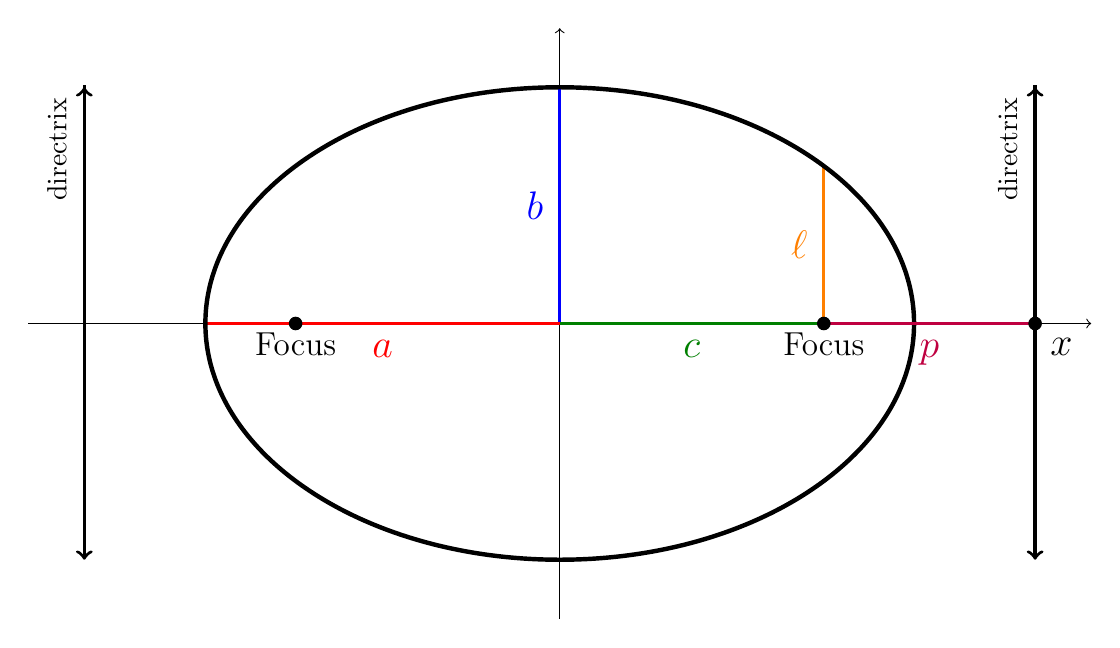
\begin{tikzpicture}[scale=3]
 %\draw[step=.5cm, gray, very thin] (-1.7,-1.2) grid (1.7,1.2); 
 \draw[->] (-2.25,0) -- (2.25,0) coordinate (x axis);
 \draw[->] (0,-1.25) -- (0,1.25) coordinate (y axis);
 

 \draw[very thick,blue] (0,0) -- (0cm,1cm) -- node[left=2pt,fill=white] {\Large{$b$}} (0,0);
 \draw[very thick,red] (0,0) -- (-1.5cm,0cm) -- node[below=2pt,fill=white] {\Large{$a$}} (0,0);
 \draw[very thick,orange] (1.118cm,0) -- (1.118cm,0.667cm) -- node[left=2pt,fill=white] {\Large{$\ell$}} (1.118cm,0);
 \draw[very thick,black!50!green] (0,0) -- (1.118cm,0) -- node[below=2pt,fill=white] {\Large{$c$}} (0,0);


 \draw[ultra thick, ->] (0,0) ellipse (1.5cm and 1cm);
 \draw[very thick,purple] (1.118cm,0) -- (2.0125cm,0cm) -- node[below=2pt] {\Large{$p$}} (1.118cm,0);
 
 \draw[very thick,black,<->] (2.0125cm,-1cm) -- (2.0125cm,1cm) -- node[left=10pt,fill=white,rotate=90] {directrix} (2.0125cm,1);
 \draw[very thick,black,<->] (-2.0125cm,-1cm) -- (-2.0125cm,1cm) -- node[left=10pt,fill=white,rotate=90] {directrix} (-2.0125cm,1);

 
 \filldraw (1.118,0) circle (.75pt) node[align=left,   below] {\large{Focus}};
 \filldraw (-1.118,0) circle (.75pt) node[align=left,   below] {\large{Focus}};
 \filldraw (2.0125,0) circle (.75pt) node[align=left,   below right = 2pt] {\Large{$x$}};
 \end{tikzpicture}
\end{document}
